\subsection{Показатель Ляпунова}    

    Для определения устойчивости аттракторов часто используется показатель Ляпунова. Зависимость этого показателя для аттракторов модели (\ref{origin}) представлена на рисунке \ref{lyapunov}. 

    \begin{figure}
        \centering
        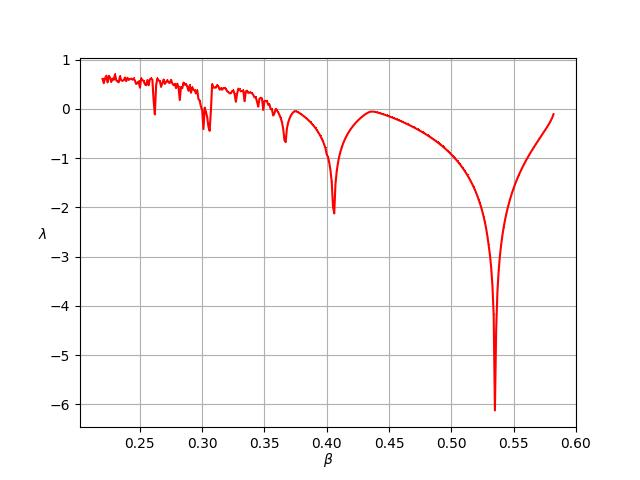
\includegraphics[width=0.8\textwidth]{deterministic/images/lyapunov.jpg}

        \captionsetup{justification=centering}
        \caption{Показатель Ляпунова для модели (\ref{origin}) при \(\alpha = 1\)}
        \label{lyapunov}
    \end{figure}

    На этом графике мы видим, что точки, где график показателя Ляпунова касается нуля точно соответствуют бифуркционным значениям, которые можно наблюдать на бифуркационной диаграмме представленной на рисунке \ref{bifurcation}.